
\documentclass[12pt,a4paper]{article}
\usepackage{geometry}
\usepackage{graphicx}
\usepackage{pythonhighlight}
\geometry{left=2.0cm,right=2.0cm,top=2.0cm,bottom=2.0cm}
\title{Week 4 Report}
\author{Zhang Heartbright}
\begin{document}
	\maketitle
	\tableofcontents
	\newpage
	\section{Part 1: Build The Functions}
		\begin{abstract}
			In this section, we will build the functions to be used for the neural network.\par
		\end{abstract}
	\subsection{1-Packages}
			\begin{python}
				import numpy as np
				import h5py
				import matplotlib.pyplot as plt
				from testCases_v3 import *
				from dnn_utils_v2 import sigmoid, sigmoid_backward, relu, relu_backward
			\end{python}
	
	\subsection{2-Outline Of Assignment}
		\begin{itemize}
			\item Initialize the parameters for a two-layer network or for an L-layer neural network.
			\item Implement the forward propagation module (shown in purple in the figure below). 
			\item Complete the LINEAR part of a layer’s forward propagation step (resulting in $Z^{[l]}$)).
			\item Use the ACTIVATION function (relu/sigmoid) provided.
			\item Combine the previous two steps into a new [LINEAR$\rightarrow$ACTIVATION] forward function.
			\item Stack the [LINEAR$\rightarrow$RELU] forward function L-1 time (for layers 1 through L-1) and add a [LINEAR$\rightarrow$SIGMOID] at the end (for the final layer L). This gives you a new L\_model\_forward function.
			\item Compute the loss and implement the backward propagation module (denoted in red in the figure below)
			\item Complete the LINEAR part of a layer’s backward propagation step.
			\item ACTIVATE function (relu\_backward/sigmoid\_backward) is given and combine the previous two steps into a new [LINEAR-ACTIVATION] backward function.
			\item Stack [LINEAR$\rightarrow$RELU] backward L-1 times and add [LINEAR$\rightarrow$SIGMOID] backward in a new L\_model\_backward function
		\end{itemize}
		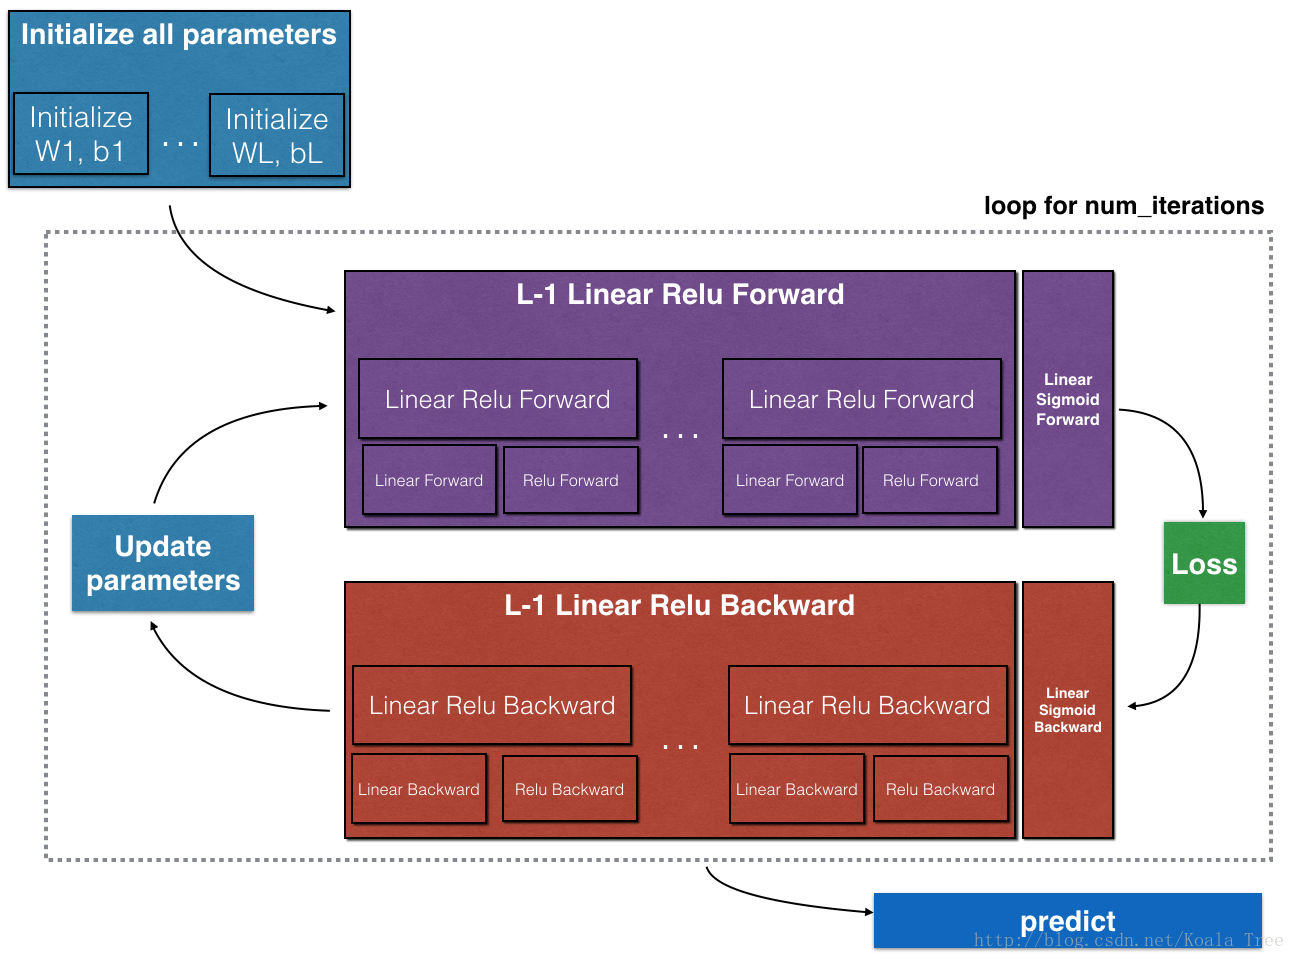
\includegraphics[scale=0.7]{image_1.png}
		\newpage
	\subsection{3-Initialization}
		\subsubsection{Two Layer Neural Network}
			\begin{itemize}
				\item The model’s structure is: LINEAR $\rightarrow$ RELU $\rightarrow$ LINEAR $\rightarrow$ SIGMOID. 
				
				\item Use random initialization for the weight matrices. Use np.random.randn(shape)*0.01 with the correct shape.
				\item Use zero initialization for the biases. Use np.zeros(shape).
				
			\end{itemize}
			\begin{python}
				def initialize_parameters(n_x, n_h, n_y):
				##--这个函数用来初始化两层神经网络的权重参数--##
				"""
				n_x -- size of the input layer
				n_h -- size of the hidden layer
				n_y -- size of the output layer
				Returns:
				parameters -- python dictionary containing your parameters:
				W1 -- weight matrix of shape (n_h, n_x)
				b1 -- bias vector of shape (n_h, 1)
				W2 -- weight matrix of shape (n_y, n_h)
				b2 -- bias vector of shape (n_y, 1)
				
				"""
				np.random.seed(1)
				###---start---###
				W1=np.random.randn(n_h,n_x)*0.01
				b1=np.zeros((n_h,1))
				W2=np.random.randn(n_y,n_h)*0.01
				b2=np.zeros((n_y,1))
				
				###---debug---###
				assert(W1.shape == (n_h, n_x))
				assert(b1.shape == (n_h, 1))
				assert(W2.shape == (n_y, n_h))
				assert(b2.shape == (n_y, 1))
				###---debug_end---###
				parameters={
					"W1":W1,
					"b1":b1,
					"W2":W2,
					"b2":b2
				}
				return parameters
			\end{python}
		\newpage
		\subsubsection{L Layer Neural Network}
			The initialization for a deeper L-layer neural network is more complicated because there are many more weight matrices and bias vectors.\par
			When computing the initialization, we should make sure that our demensions math in each layer\par
			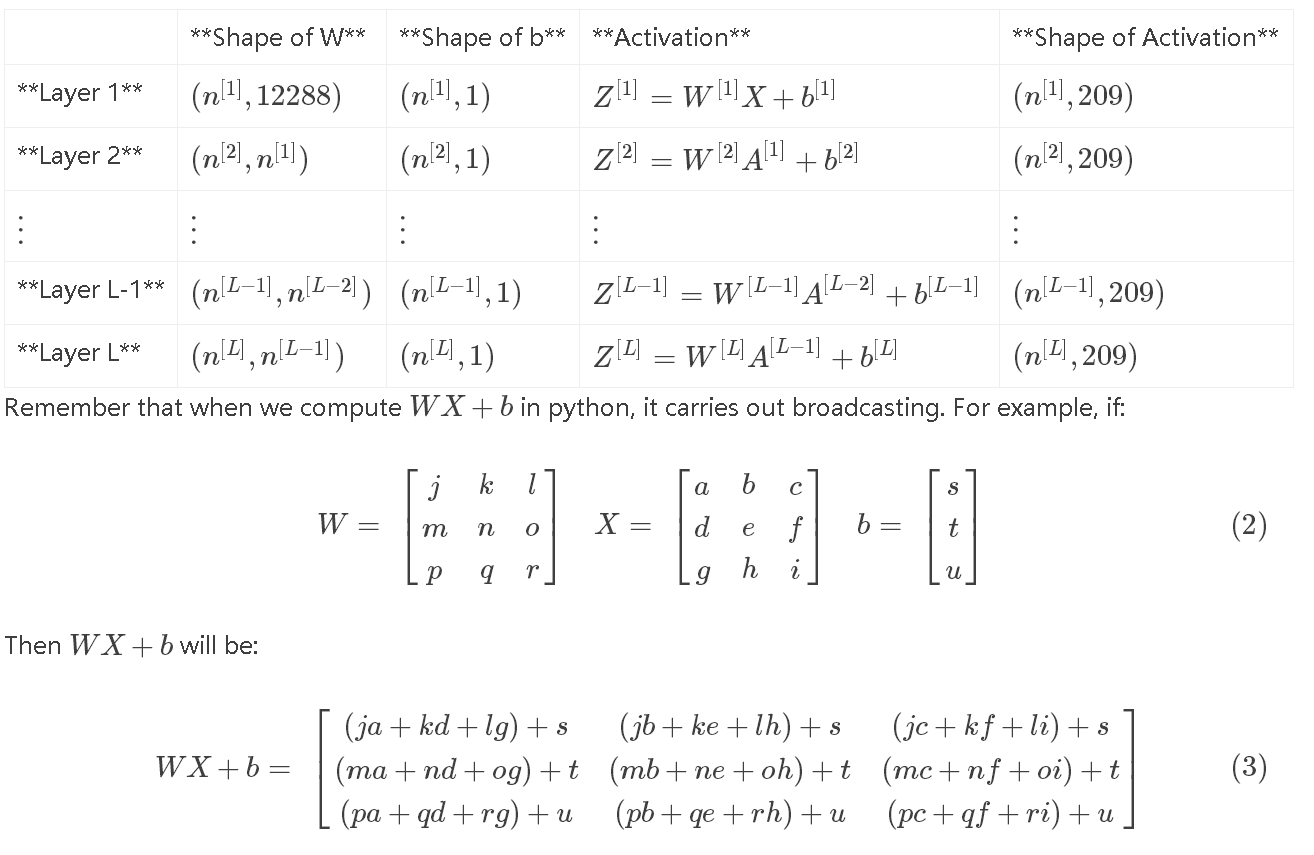
\includegraphics[scale=0.7]{image_2.png}
			\begin{itemize}
				\item Use random initialization for the weight matrices.
				\item Use zeros initialization for the biases.
				\item We will store $n^{[l]}$, the number of units in different layers, in a variable layer\_dims. 
				\item The following  is the implementation for L=1, which can implement the general cases.
			\end{itemize}
		\newpage
			\begin{python}
				def initialize_parameters_deep(layer_dims):
				"""
				Arguments:
				layer_dims -- python array (list) containing the dimensions of each layer in our network
				
				Returns:
				parameters -- python dictionary containing your parameters "W1", "b1", ..., "WL", "bL":
				Wl -- weight matrix of shape (layer_dims[l], layer_dims[l-1])
				bl -- bias vector of shape (layer_dims[l], 1)
				"""
				np.random.seed(3)
				parameters={}
				L=len(layer_dims)
				
				for l in range(1,L):
				parameters['W'+str(l)]=np.random.randn(layer_dims[l],layer_dims[l-1])*0.01
				parameters['b'+str(l)]=np.zeros((layer_dims[l],1))
				assert(parameters['W'+str(l)].shape==(layer_dims[l],layer_dims[l-1]))
				assert(parameters['b'+str(l)].shape==(layer_dims[l],1))
				return parameters
			\end{python}
			\newpage
	\subsection{4-Forward Propogation}
		\subsubsection{Linear Forward}
			\begin{itemize}
				\item LINEAR
				\item LINEAR $\rightarrow$ ACTIVATION where ACTIVATION will be either ReLU or Sigmoid.
				\item (LINEAR - RELU) × (L-1) $\rightarrow$ LINEAR $\rightarrow$ SIGMOID (whole model)				
			\end{itemize}
			$Z^{[L]}=W^{[L]}A^{[L-1]}$\par
			where $A^{[0]}=X$
			\newpage
			\begin{python}
				def linear_forward(A,W,b):
				"""
				Implement the linear part of a layer's forward propagation.
				
				Arguments:
				A -- activations from previous layer (or input data): (size of previous layer, number of examples)
				W -- weights matrix: numpy array of shape (size of current layer, size of previous layer)
				b -- bias vector, numpy array of shape (size of the current layer, 1)
				
				Returns:
				Z -- the input of the activation function, also called pre-activation parameter
				cache -- a python dictionary containing "A", "W" and "b" ; stored for computing the backward pass efficiently
				"""
				###---start---###
				Z=np.dot(W,A)+b
				###---end---###
				assert(Z.shape==(W.shape[0],A.shape[1]))
				cache=(A,W,b)
				
				return Z,cache
			\end{python}
		\newpage
		\subsubsection{Linear-Activation Forward}
			The functions to be used:
			\begin{itemize}
				\item Sigmoid: $\delta(Z)=\delta(WA+b)=\frac{1}{1+e^{-WA+b}}$
				\item Relu:
				$ A=RELU(Z)=max(0,Z)$
			\end{itemize}
			\begin{python}
				def linear_activation_forward(A_prev, W, b, activation):
				"""
				Implement the forward propagation for the LINEAR->ACTIVATION layer
				
				Arguments:
				A_prev -- activations from previous layer (or input data): (size of previous layer, number of examples)
				W -- weights matrix: numpy array of shape (size of current layer, size of previous layer)
				b -- bias vector, numpy array of shape (size of the current layer, 1)
				activation -- the activation to be used in this layer, stored as a text string: "sigmoid" or "relu"
				
				Returns:
				A -- the output of the activation function, also called the post-activation value
				cache -- a python dictionary containing "linear_cache" and "activation_cache";
				stored for computing the backward pass efficiently
				
				"""
				###---start---###
				if activation =="sigmoid":#判断是哪个激活函数
				Z,linear_cache=linear_forward(A_prev,W,b)#linear_cache 对应A_prev,W,b是Z=WX+b里的X,W和b
				A,activation_cache=sigmoid(Z)#cache is Z
				
				elif activation =="relu":
				Z,linear_cache=linear_forward(A_prev,W,b)
				A,activation_cache=relu(Z)
				###---end---###
				assert(A.shape==(W.shape[0],A_prev.shape[1]))
				cache=(linear_cache,activation_cache)
				return A,cache
			\end{python}
		\newpage
		\subsubsection{L-Layer Model Forward}
		The function to be used:
			\begin{itemize}
				\item $A^{[L]}=\delta(Z)=\delta(W^{[l]}A^{[L-1]}+b^{[L]})$
			\end{itemize}
			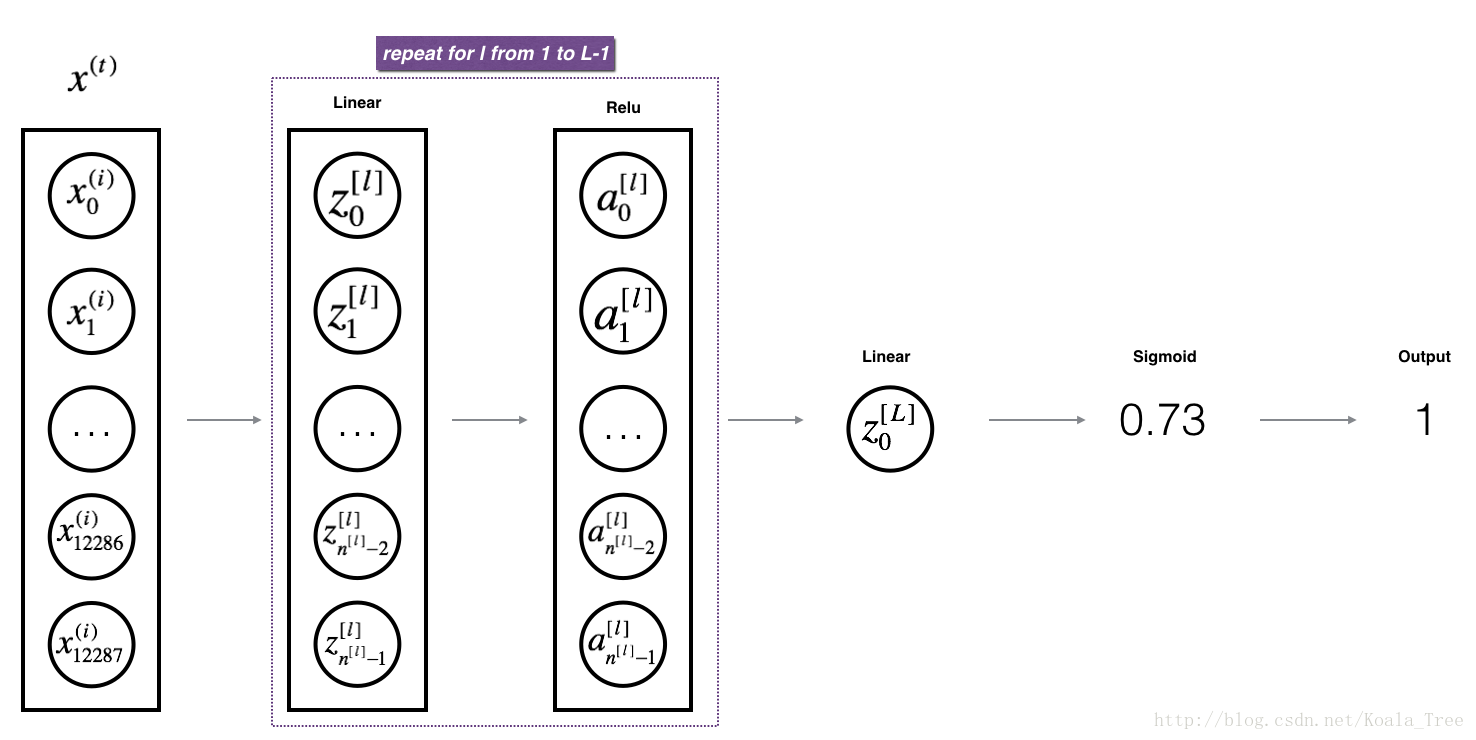
\includegraphics[scale=0.6]{image_3.png}
			\newpage
			\begin{python}
				def L_model_forward(X, parameters):
				"""
				Implement forward propagation for the [LINEAR->RELU]*(L-1)->LINEAR->SIGMOID computation

				Arguments:
				X -- data, numpy array of shape (input size, number of examples)
				parameters -- output of initialize_parameters_deep()
				
				Returns:
				AL -- last post-activation value
				caches -- list of caches containing:
				every cache of linear_relu_forward() (there are L-1 of them, indexed from 0 to L-2)
				the cache of linear_sigmoid_forward() (there is one, indexed L-1)
				"""
				
				caches = []
				A = X
				L = len(parameters) // 2 # number of layers in the neural network
				#这里面只有 w和b,所以parameters需要整除2
				# Implement [LINEAR -> RELU]*(L-1). Add "cache" to the "caches" list.
				for l in range(1, L):#循环从L到L-1
				A_prev = A
				###---start---###
				A,cache=linear_activation_forward(A_prev,W=parameters['W'+str(l)],b=parameters['b'+str(l)],activation="relu")
				caches.append(cache)
				###---end---###
				
				# Implement LINEAR -> SIGMOID. Add "cache" to the "caches" list.
				###---start---### (≈ 2 lines of code)
				AL,cache=linear_activation_forward(A,W=parameters['W'+str(L)],b=parameters['b'+str(L)],activation="sigmoid")
				caches.append(cache)
				###---end---###
				
				assert(AL.shape == (1,X.shape[1]))
				
				return AL, caches
			\end{python}
		\newpage
	\subsection{5-Cost Function}
	The cost function is used to check if the model is really learning\par
	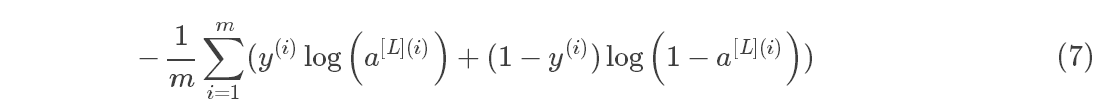
\includegraphics[scale=0.8]{image_4.png}
	\begin{python}
		def compute_cost(AL, Y):
		"""
		Implement the cost function defined by equation (7).
		
		Arguments:
		AL -- probability vector corresponding to your label predictions, shape (1, number of examples)
		Y -- true "label" vector (for example: containing 0 if non-cat, 1 if cat), shape (1, number of examples)
		
		Returns:
		cost -- cross-entropy cost
		"""
		
		m = Y.shape[1]
		
		# Compute loss from aL and y.
		###---start---### (≈ 1 lines of code)
		cost=-np.sum(np.multiply(np.log(AL),Y)+np.multiply(np.log(1-AL),1-Y))/m
		###---end---###
		
		cost = np.squeeze(cost) # To make sure your cost's shape is what we expect (e.g. this turns [[17]] into 17).
		assert(cost.shape == ())
		
		return cost
	\end{python}
	\subsection{6-Backward Propogation}
		We use a picture to illustrate it:\par
		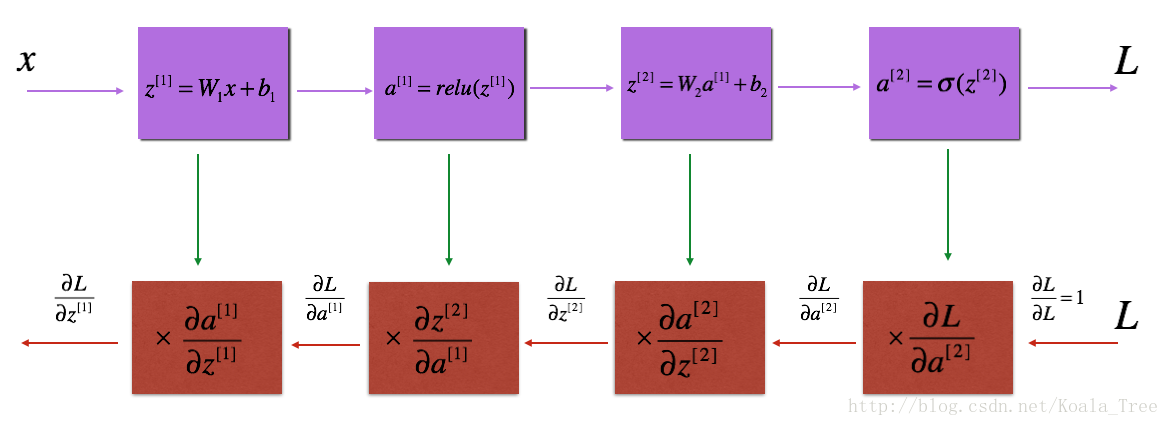
\includegraphics[scale=0.7]{image_5.png}\par
		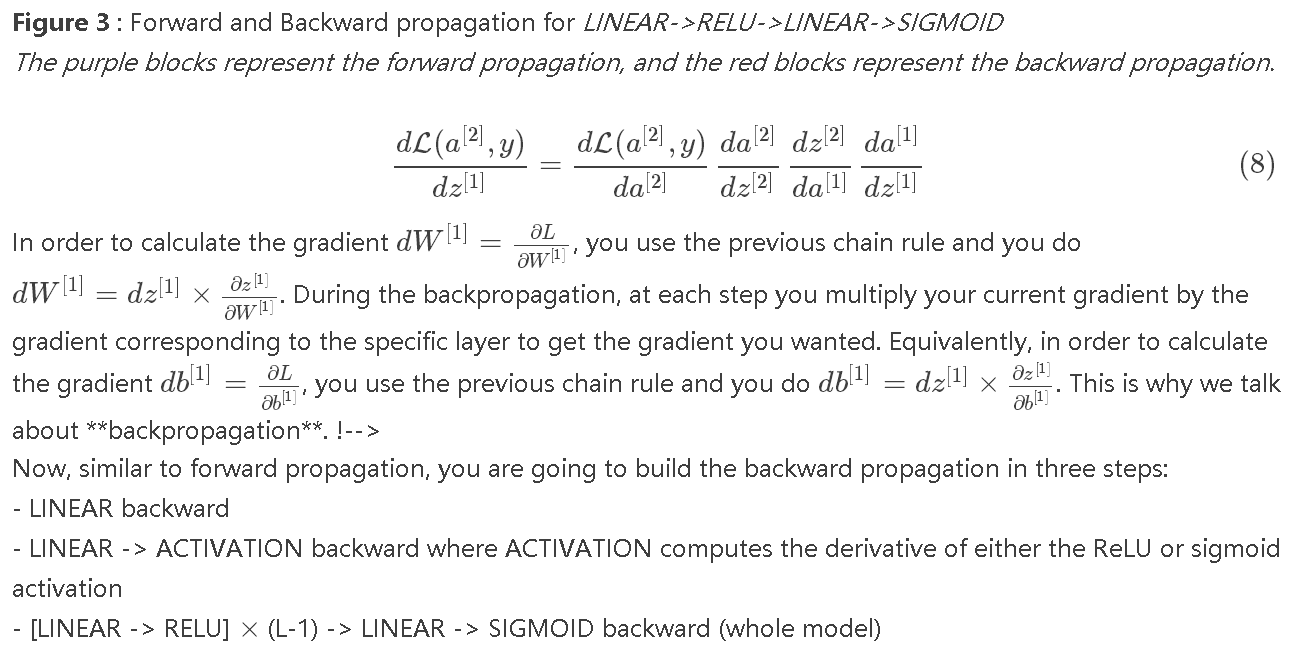
\includegraphics[scale=0.7]{image_6.png}\par

			\subsubsection{Linear backward}
				\begin{itemize}
					\item For layer l, the linear part is: $Z^{[L]}=W^{[L]}A^{[L-1]}+b^{[l]}$\par
				\end{itemize}
		\qquad\qquad\qquad\qquad\qquad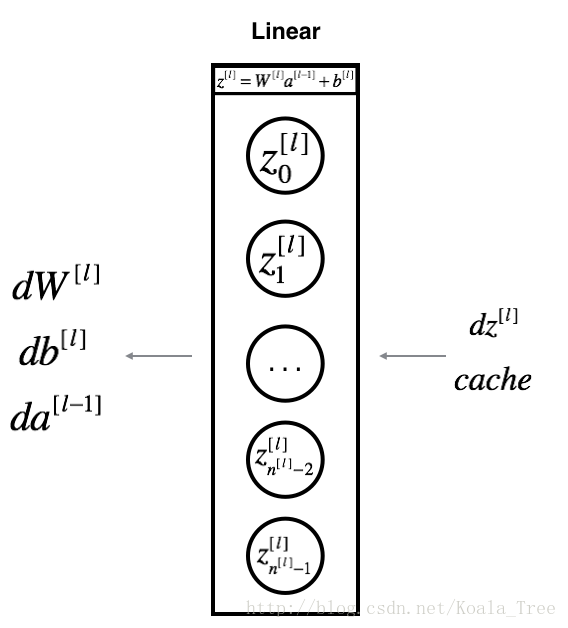
\includegraphics[scale=0.8]{image_7.png}\par
		To compute dW,db,da :\par
		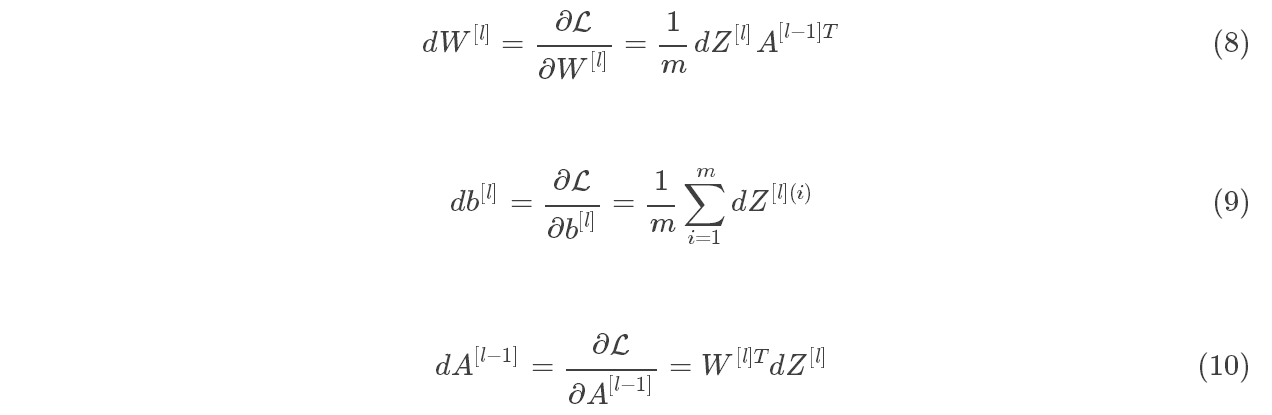
\includegraphics[scale=0.6]{image_8.png}
		\newpage
		\begin{python}
			def linear_backward(dZ, cache):
			"""
			Implement the linear portion of backward propagation for a single layer (layer l)
			
			Arguments:
			dZ -- Gradient of the cost with respect to the linear output (of current layer l)
			cache -- tuple of values (A_prev, W, b) coming from the forward propagation in the current layer
			
			Returns:
			dA_prev -- Gradient of the cost with respect to the activation (of the previous layer l-1), same shape as A_prev
			dW -- Gradient of the cost with respect to W (current layer l), same shape as W
			db -- Gradient of the cost with respect to b (current layer l), same shape as b
			"""
			
			A_prev, W, b = cache
			m = A_prev.shape[1]
			
			###---start---###
			dW=np.dot(dZ,A_prev.T)/m
			db=np.sum(dZ,axis=1,keepdims=True)#axis是遍历间隔,keepdims是持续迭代
			dA_prev=np.dot(W.T,dZ)
			###---end---###
			
			assert (dA_prev.shape == A_prev.shape)
			assert (dW.shape == W.shape)
			assert (db.shape == b.shape)
			
			return dA_prev, dW, db
			
		\end{python}
	\newpage
		\subsubsection{Linear-Activation backward}
			In this section we create a function that merges the two helper functions: linear\_backward and the backward step for the activation linear\_activation\_backward.\par
			And the codes are as followings:\par
			\begin{python}
				def linear_activation_backward(dA, cache, activation):
				"""
				Implement the backward propagation for the LINEAR->ACTIVATION layer.
				
				Arguments:
				dA -- post-activation gradient for current layer l
				cache -- tuple of values (linear_cache, activation_cache) we store for computing backward propagation efficiently
				activation -- the activation to be used in this layer, stored as a text string: "sigmoid" or "relu"
				
				Returns:
				dA_prev -- Gradient of the cost with respect to the activation (of the previous layer l-1), same shape as A_prev
				dW -- Gradient of the cost with respect to W (current layer l), same shape as W
				db -- Gradient of the cost with respect to b (current layer l), same shape as b
				"""
				linear_cache, activation_cache = cache
				
				if activation == "relu":
				###---start---### 
				dZ=relu_backward(dA,activation_cache)
				dA_prev,dW,db=linear_backward(dZ,linear_cache)
				###---end---###
				
				elif activation == "sigmoid":
				###---start---### 
				dZ=sigmoid_backward(dA,activation_cache)
				dA_prev,dW,db=linear_backward(dZ,linear_cache)
				###---end---###
				
				return dA_prev, dW, db
			\end{python}
		\newpage
		\subsubsection{L-Model Backward}
		\begin{itemize}
			\item Now we can implement the backward function for the whole network.
			\item On each step, we use the cached values for layer l to backpropagate through layer l
		\end{itemize}
		\qquad\qquad\quad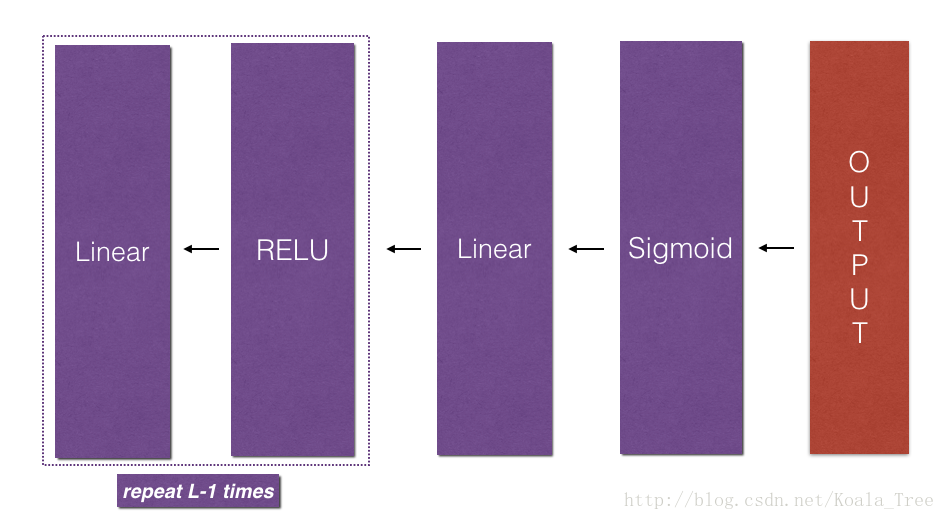
\includegraphics[scale=0.8]{image_9}
		\newpage
		\begin{python}
			def L_model_backward(AL, Y, caches):
			"""
			Implement the backward propagation for the [LINEAR->RELU] * (L-1) -> LINEAR -> SIGMOID group
			
			Arguments:
			AL -- probability vector, output of the forward propagation 
			
			(L_model_forward())
			Y -- true "label" vector (containing 0 if non-cat, 1 if cat)
			caches -- list of caches containing:
			every cache of linear_activation_forward() with "relu" 
			(it's caches[l], for l in range(L-1) i.e l = 0...L-2)
			the cache of linear_activation_forward() with "sigmoid" 
			(it's caches[L-1])
			
			Returns:
			grads -- A dictionary with the gradients
			grads["dA" + str(l)] = ...
			grads["dW" + str(l)] = ...
			grads["db" + str(l)] = ...
			"""
			grads = {}
			L = len(caches) # the number of layers
			Y = Y.reshape(AL.shape) # after this line, Y is the same shape as AL
			
			# Initializing the backpropagation
			###---start---### (1 line of code)
			dAL=-Y/AL +(1-Y)/(1-AL)
			###---end---###
			
			# Lth layer (SIGMOID -> LINEAR) gradients. """
			Inputs: "AL, Y, caches". 
			Outputs: "grads["dAL"], grads["dWL"], grads["dbL"]
			"""
			###---start---### (approx. 2 lines)
			current_cache=caches[L-1]
			grads["dA"+str(L)],grads["dW"+str(L)],grads["db"+str(L)]=
			linear_activation_backward(dAL,current_cache,activation="sigmoid")
			###---end---###
			
			for l in reversed(range(L-1)):
			# lth layer: (RELU -> LINEAR) gradients.
			# Inputs: "grads["dA" + str(l + 2)], caches". 
			# Outputs: "grads["dA" + str(l + 1)] , grads["dW" + str(l + 1)] , grads["db" + str(l + 1)]
			
			###---start---### (approx. 5 lines)
			print(l)
			current_cache=caches[l]
			dA_prev_t,dW_t,db_t=linear_activation_backward(dA=grads["dA"+str(l+2)],cache=current_cache,activation="relu")
			grads["dA"+str(l+1)]=dA_prev_t
			grads["dW"+str(l+1)]=dW_t
			grads["db"+str(l+1)]=db_t        
			###---end---###
			
			return grads
		\end{python}
		\subsubsection{Update Parameters}
		In this section we use grad-decents to update the parameters.\par Functions are as follows:\par
		\begin{itemize}
			\item $W^{[l]}=W^{[l]}−α dW^{[l]}    $
			\item $b^{[l]}=b^{[l]}−α db^{[l]}    $
		\end{itemize}
	\section{Part 2: Build A Two Layer Neural Network}
		\begin{abstract}
			This time, we can use the models above to make a 2-layer neural network
		\end{abstract}
		\begin{python}
			#this is a 2-layer network
			# And we use the codes we have done before
			import time
			import numpy as np
			import h5py
			import matplotlib.pyplot as plt
			import scipy
			from PIL import Image
			from scipy import ndimage
			from dnn_app_utils_v2 import *
			""" 前期数据准备 """
			np.random.seed(2)
			train_x_orign,train_y,test_x_orign,test_y,classes=load_data()
			#print("train_x_orign shape: "+ str(train_x_orign.shape))
			train_x_flatten=train_x_orign.reshape(train_x_orign.shape[0],-1).T 
			#after flatten:(12288,209)
			test_x_flatten=test_x_orign.reshape(test_x_orign.shape[0],-1).T 
			#after flatten:(12288,209)
			###---standarlize---###
			train_x=train_x_flatten/255.
			test_x=test_x_flatten/255.
			
			###---内容决定了是几层网络---####
			n_x = 12288 # num_px * num_px * 3
			n_h = 7     # 隐藏层有7个单元
			n_y = 1     # 输出有一个
			layers_dims = (n_x, n_h, n_y)
			"""
			Argument:
			n_x -- size of the input layer
			n_h -- size of the hidden layer
			n_y -- size of the output layer
			"""
			
			#############################
			###- - - - - - - - - - - -###
			###- - B I G S T A R T - -###
			###- - - - - - - - - - - -###
			#############################
			
			
			###---2层神经网络---###
			def two_layer_model(X, Y, layers_dims, learning_rate = 0.0075, num_iterations = 3000, print_cost=False):
			"""
			Implements a two-layer neural network: LINEAR->RELU->LINEAR->SIGMOID.
			
			Arguments:
			X -- input data, of shape (n_x, number of examples)
			Y -- true "label" vector (containing 0 if cat, 1 if non-cat), of shape (1, number of examples)
			layers_dims -- dimensions of the layers (n_x, n_h, n_y)
			num_iterations -- number of iterations of the optimization loop
			learning_rate -- learning rate of the gradient descent update rule
			print_cost -- If set to True, this will print the cost every 100 iterations
			
			Returns:
			parameters -- a dictionary containing W1, W2, b1, and b2
			"""
			
			np.random.seed(1)
			grads = {}
			costs = [] # to keep track of the cost
			m = X.shape[1] # number of examples
			(n_x, n_h, n_y) = layers_dims
			
			# Initialize parameters dictionary, by calling one of the functions you'd previously implemented
			# 初始化参数
			###---start---### (≈ 1 line of code)
			parameters = initialize_parameters(n_x, n_h, n_y)
			###---end---###
			
			# Get W1, b1, W2 and b2 from the dictionary parameters.
			W1 = parameters["W1"]
			b1 = parameters["b1"]
			W2 = parameters["W2"]
			b2 = parameters["b2"]
			
			# Loop (gradient descent)
			
			for i in range(0, num_iterations):
			#前向传播
			# Forward propagation: LINEAR -> RELU -> LINEAR -> SIGMOID. Inputs: "X, W1, b1". Output: "A1, cache1, A2, cache2".
			###---start---### (≈ 2 lines of code)
			# A1, cache1 = linear_activation_forward(X, W1, b1, activation="relu")
			# A2, cache2 = linear_activation_forward(A1, W2, b2, activation="sigmoid")
			A1,cache1=linear_activation_forward(A_prev=X,W=W1,b=b1,activation="relu")
			A2,cache2=linear_activation_forward(A_prev=A1,W=W2,b=b2,activation="sigmoid")
			###---end---###
			
			# 计算成本函数
			###---start---### (≈ 1 line of code)
			#cost = compute_cost(A2, Y)
			cost=compute_cost(AL=A2,Y=Y)
			###---end---###
			
			# Initializing backward propagation
			#初始化反向传播
			#dA2 = - (np.divide(Y, A2) - np.divide(1 - Y, 1 - A2))
			dA2=-(Y/A2  - (1-Y)/1-A2)
			
			# Backward propagation. Inputs: "dA2, cache2, cache1". Outputs: "dA1, dW2, db2; also dA0 (not used), dW1, db1".
			#反向传播
			###---start---### (≈ 2 lines of code)
			# dA1, dW2, db2 = linear_activation_backward(dA2, cache2, activation="sigmoid")
			# dA0, dW1, db1 = linear_activation_backward(dA1, cache1, activation="relu")
			dA1,dW2,db2=linear_activation_backward(dA=dA2,cache=cache2,activation="sigmoid")
			dA0,dW1,db1=linear_activation_backward(dA=dA1,cache=cache1,activation="relu")
			###---end---###
			
			# Set grads['dWl'] to dW1, grads['db1'] to db1, grads['dW2'] to dW2, grads['db2'] to db2
			#设置梯度
			grads['dW1'] = dW1
			grads['db1'] = db1
			grads['dW2'] = dW2
			grads['db2'] = db2
			
			# Update parameters.
			# 更新参数
			###---start---### (approx. 1 line of code)
			#parameters = update_parameters(parameters, grads, learning_rate)
			parameters=update_parameters(parameters,grads,learning_rate)
			###---end---###
			
			# Retrieve W1, b1, W2, b2 from parameters
			# 替换更新
			W1 = parameters["W1"]
			b1 = parameters["b1"]
			W2 = parameters["W2"]
			b2 = parameters["b2"]
			
			# Print the cost every 100 training example
			# 每一百次学习查看成本损失
			
			if print_cost and i % 100 == 0:
			print("Cost after iteration {}: {}".format(i, np.squeeze(cost)))
			# if print_cost and i % 100 == 0:
			costs.append(cost)
			
			# plot the cost
			
			plt.plot(np.squeeze(costs))
			plt.ylabel('cost')
			plt.xlabel('iterations (per tens)')
			plt.title("Learning rate =" + str(learning_rate))
			plt.show()
			
			return parameters
			# 运行模型
			
			#parameters = two_layer_model(train_x, train_y, layers_dims = (n_x, n_h, n_y), num_iterations = 2500, print_cost=True)
			parameters=two_layer_model(train_x,train_y,learning_rate=0.0075,layers_dims=(n_x,n_h,n_y),num_iterations=2000,print_cost=True)
			predictions_train = predict(train_x, train_y, parameters)
			predictions_test = predict(test_x, test_y, parameters)
		\end{python}
		part of the results:\par
		\begin{python}
			Cost after iteration 0: 0.693049735659989
			Cost after iteration 100: 0.6482760951508908
			Cost after iteration 200: 0.638429336340072
			Cost after iteration 300: 0.6178888768868509
			Cost after iteration 400: 0.5836516666225391
			Cost after iteration 500: 0.5449045395510413
			Cost after iteration 600: 0.5054427467790368
			Cost after iteration 700: 0.47074581506515784
			Cost after iteration 800: 0.4381328874628742
			Cost after iteration 900: 0.42283406420844005
			Cost after iteration 1000: 0.405879611011641
			Cost after iteration 1100: 0.3717984866548225
			Cost after iteration 1200: 0.3416123497167632
			Cost after iteration 1300: 0.2926623715470592
			Cost after iteration 1400: 0.2686173406673315
			Cost after iteration 1500: 0.2344362805323333
			Cost after iteration 1600: 0.20941723048656552
			Cost after iteration 1700: 0.19027892302796698
			Cost after iteration 1800: 0.1736818636718253
			Cost after iteration 1900: 0.160404331880999
		\end{python}
		the analysis:
		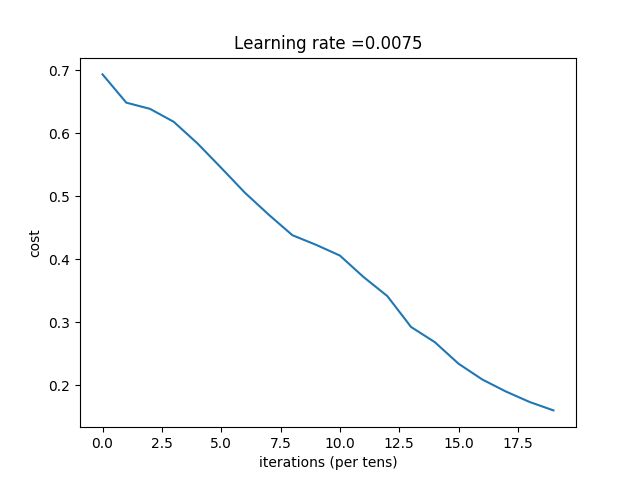
\includegraphics[scale=0.8]{Figure_1.png}
	\section{Part 3: Build A L-layer Neural Network}
	 No explain, just similiar as before.\par
	 \begin{python}
	 	#this is a 5-layer network
	 	# And we use the codes we have done before
	 	import time
	 	import numpy as np
	 	import h5py
	 	import matplotlib.pyplot as plt
	 	import scipy
	 	from PIL import Image
	 	from scipy import ndimage
	 	from dnn_app_utils_v2 import *
	 	
	 	np.random.seed(1)
	 	
	 	train_x_orign,train_y,test_x_orign,test_y,classes=load_data()
	 	
	 	train_x_flatten=train_x_orign.reshape(train_x_orign.shape[0],-1).T 
	 	#print(format(train_x_flatten.shape))# (12288,209)
	 	test_x_flatten=test_x_orign.reshape(test_x_orign.shape[0],-1).T 
	 	#print(format(test_x_flatten.shape))#(12288,50)
	 	###---standarlize---###
	 	train_x=train_x_flatten/255
	 	test_x=test_x_flatten/255
	 	
	 	layers_dims = [12288, 20, 7, 5, 1] # 5-layer model
	 	
	 	#############################
	 	###- - - - - - - - - - - -###
	 	###- - B I G S T A R T - -###
	 	###- - - - - - - - - - - -###
	 	#############################
	 	
	 	def L_layer_model(X, Y, layers_dims, learning_rate = 0.0075, num_iterations = 3000, print_cost=False):#lr was 0.009
	 	"""
	 	Implements a L-layer neural network: [LINEAR->RELU]*(L-1)->LINEAR->SIGMOID.
	 	
	 	Arguments:
	 	X -- data, numpy array of shape (number of examples, num_px * num_px * 3)
	 	Y -- true "label" vector (containing 0 if cat, 1 if non-cat), of shape (1, number of examples)
	 	layers_dims -- list containing the input size and each layer size, of length (number of layers + 1).
	 	learning_rate -- learning rate of the gradient descent update rule
	 	num_iterations -- number of iterations of the optimization loop
	 	print_cost -- if True, it prints the cost every 100 steps
	 	
	 	Returns:
	 	parameters -- parameters learnt by the model. They can then be used to predict.
	 	"""
	 	
	 	np.random.seed(1)
	 	costs = [] # keep track of cost
	 	
	 	# Parameters initialization.
	 	###---start---###
	 	# parameters = initialize_parameters_deep(layers_dims)
	 	parameters=initialize_parameters_deep(layers_dims)
	 	###---end---###
	 	
	 	# Loop (gradient descent)
	 	for i in range(0, num_iterations):
	 	
	 	# Forward propagation: [LINEAR -> RELU]*(L-1) -> LINEAR -> SIGMOID.
	 	###---start---### (≈ 1 line of code)
	 	# AL, caches = L_model_forward(X, parameters)
	 	A_last,caches=L_model_forward(X=X,parameters=parameters)
	 	###---end---###
	 	
	 	# Compute cost.
	 	###---start---### (≈ 1 line of code)
	 	# cost = compute_cost(AL, Y)
	 	cost=compute_cost(AL=A_last,Y=Y)
	 	###---end---###
	 	
	 	# Backward propagation.
	 	###---start---### (≈ 1 line of code)
	 	# grads = L_model_backward(AL, Y, caches)
	 	grads=L_model_backward(AL=A_last,Y=Y,caches=caches)
	 	###---end---###
	 	
	 	# Update parameters.
	 	###---start---### (≈ 1 line of code)
	 	# parameters = update_parameters(parameters, grads, learning_rate)
	 	parameters=update_parameters(parameters=parameters,learning_rate=learning_rate,grads=grads)
	 	###---end---###
	 	
	 	# Print the cost every 100 training example
	 	if print_cost and i % 100 == 0:
	 	print ("Cost after iteration {}:{}" .format(i,np.squeeze(cost)))
	 	#if print_cost and i % 100 == 0:
	 	costs.append(cost)
	 	
	 	# plot the cost
	 	plt.plot(np.squeeze(costs))
	 	plt.ylabel('cost')
	 	plt.xlabel('iterations (per tens)')
	 	plt.title("Learning rate =" + str(learning_rate))
	 	plt.show()
	 	
	 	return parameters
	 	parameters=L_layer_model(train_x,train_y,layers_dims,learning_rate=0.0075,num_iterations=2500,print_cost=True)
	 	
	 	predict(train_x,train_y,parameters)
	 	predict(test_x,test_y,parameters)
	 \end{python}
 		result analysis:\par
 		
	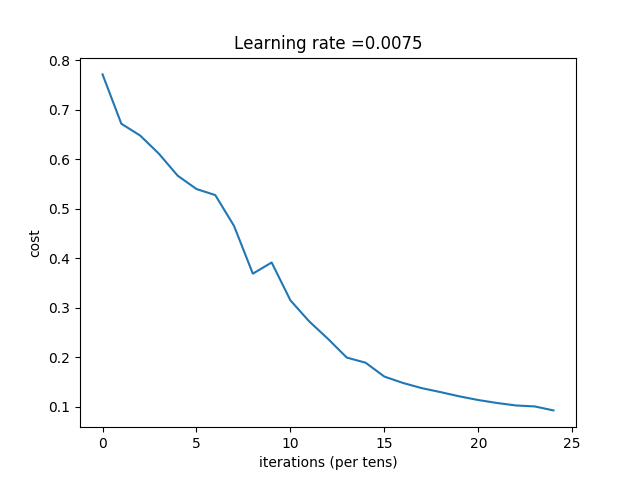
\includegraphics[]{Figure2_1.png}
 	
\end{document}